\documentclass[a4paper,12pt]{article}
\usepackage{amsmath}
\usepackage{graphicx}
\usepackage{float}
\title{Computerized Simulation \\
Exercise No. 3}
\author{name : Seyed Mohammad Ghoreishy \\ teacher : Seyed Amirhossein Tabatabaei }
\date{Date: 1403.09.26}
\begin{document}
\maketitle
\tableofcontents 
\newpage

\section{Exercise 1}
Write a program using the \textbf{accept-reject method} to generate random numbers following a custom probability distribution defined by the piecewise function as follows:
\begin{equation*}
    f(x) = \begin{cases} 
    2x & 0 \leq x \leq 0.5 \\
    2(1 - x) & 0.5 < x \leq 1.
    \end{cases}
\end{equation*}
\begin{figure}[h!]
    \centering
    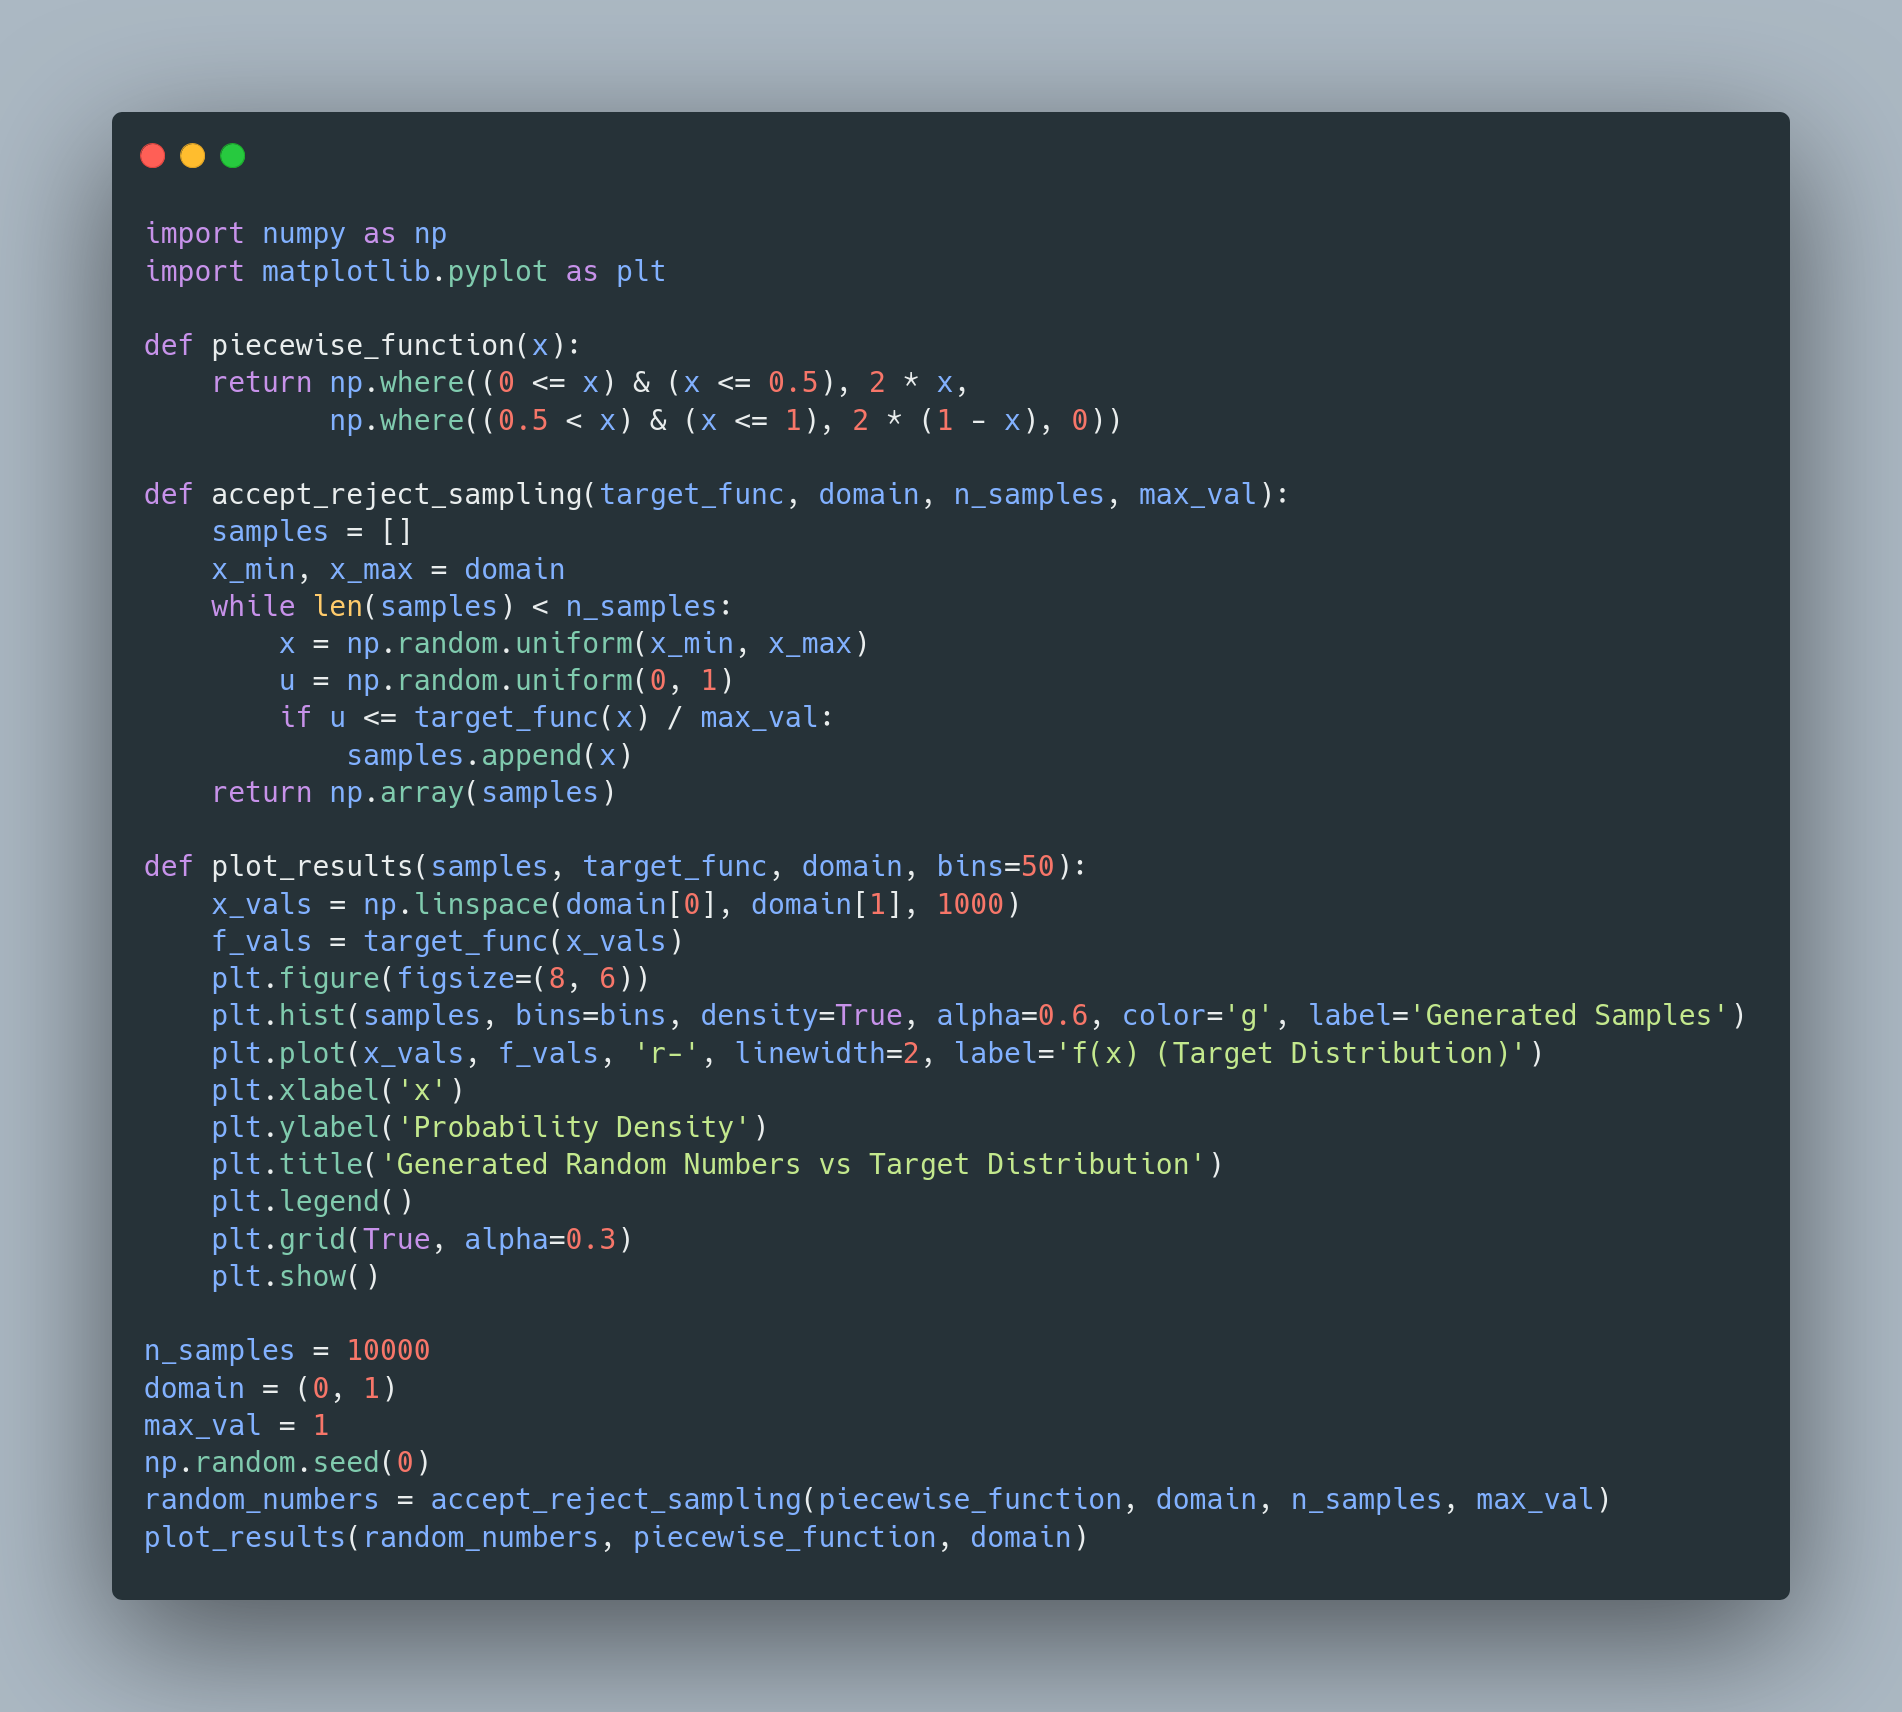
\includegraphics[width=0.6\textwidth]{./Screenshots/1.py.png} 
\end{figure} \\
\begin{figure}[h!]
    \centering
    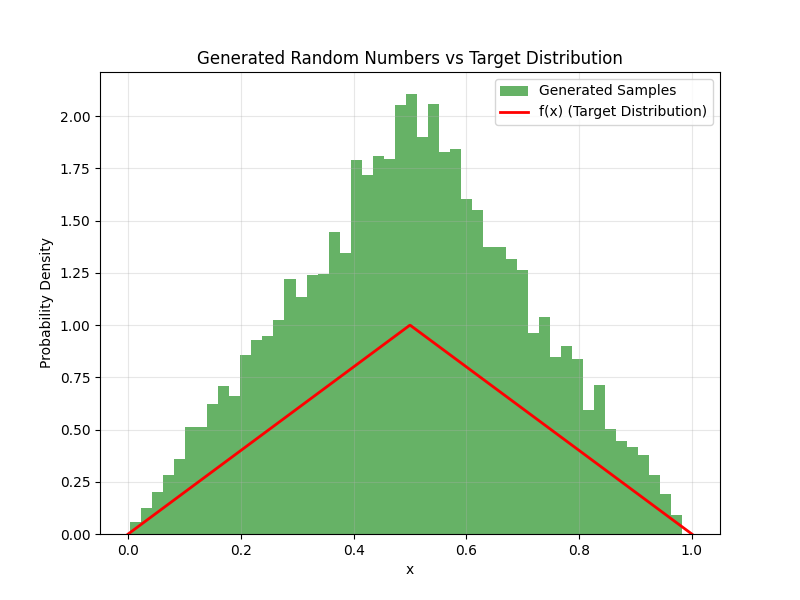
\includegraphics[width=0.6\textwidth]{./Screenshots/1.png} 
\end{figure} 
\newpage

\section{Exercise 2}
Simulate the distribution of angles at which particles scatter when the probability distribution of scattering angles is proportional to $\cos^2(x)$. Use the \textbf{accept-reject method} to generate the angles.
\begin{figure}[h!]
    \centering
    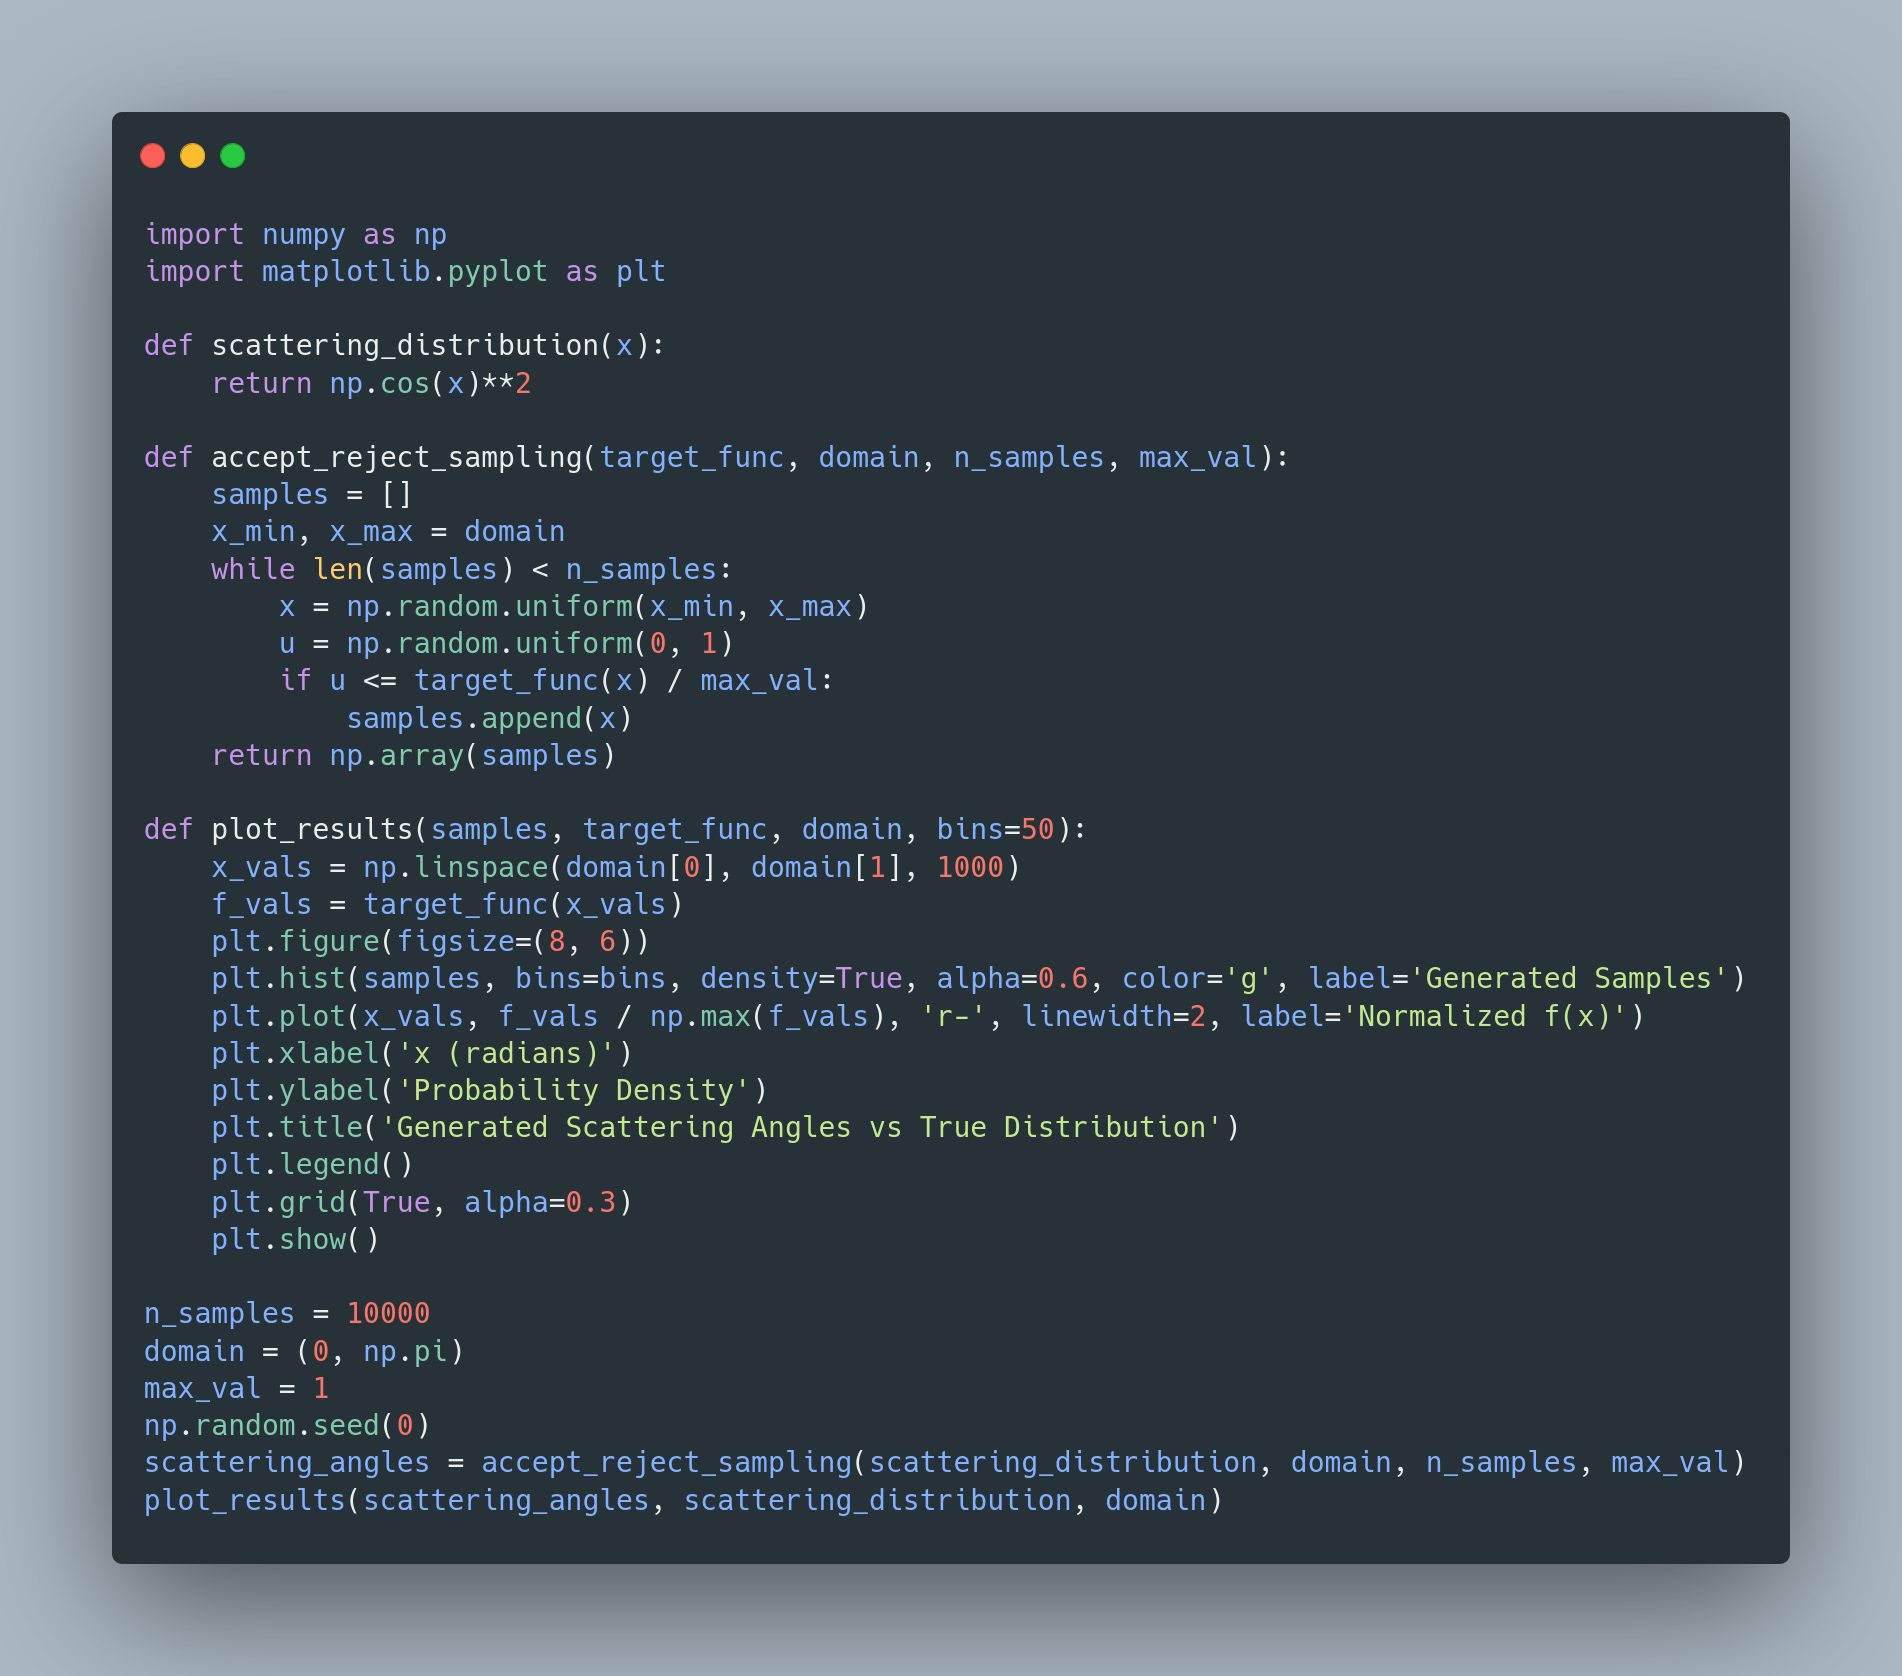
\includegraphics[width=0.6\textwidth]{./Screenshots/2.py.png} 
\end{figure} \\
\begin{figure}[h!]
    \centering
    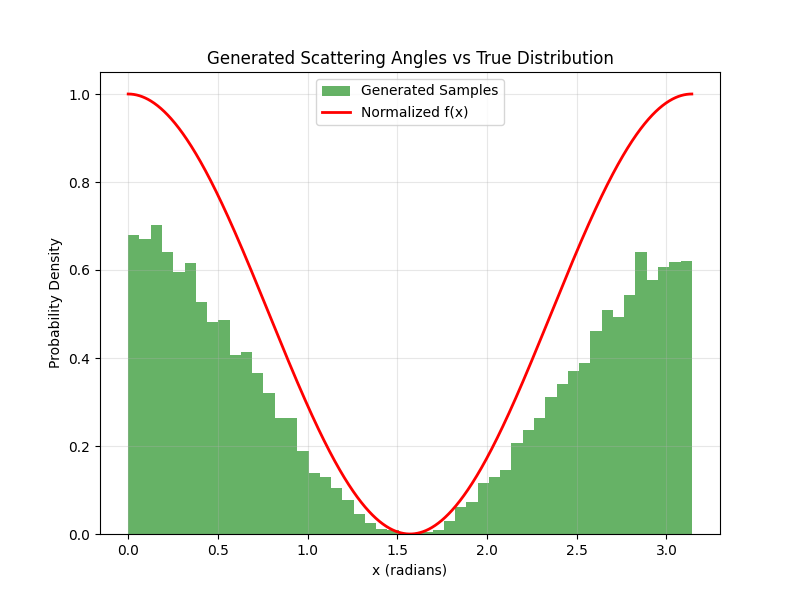
\includegraphics[width=0.6\textwidth]{./Screenshots/2.png} 
\end{figure} 
\newpage

\section{Exercise 3}
Simulate service times for customers in a queue. Assume service times follow a specific distribution (e.g., $f(x) = x e^{-x}$), and use the \textbf{accept-reject method} to generate the times. Analyze the average waiting time.
\begin{figure}[h!]
    \centering
    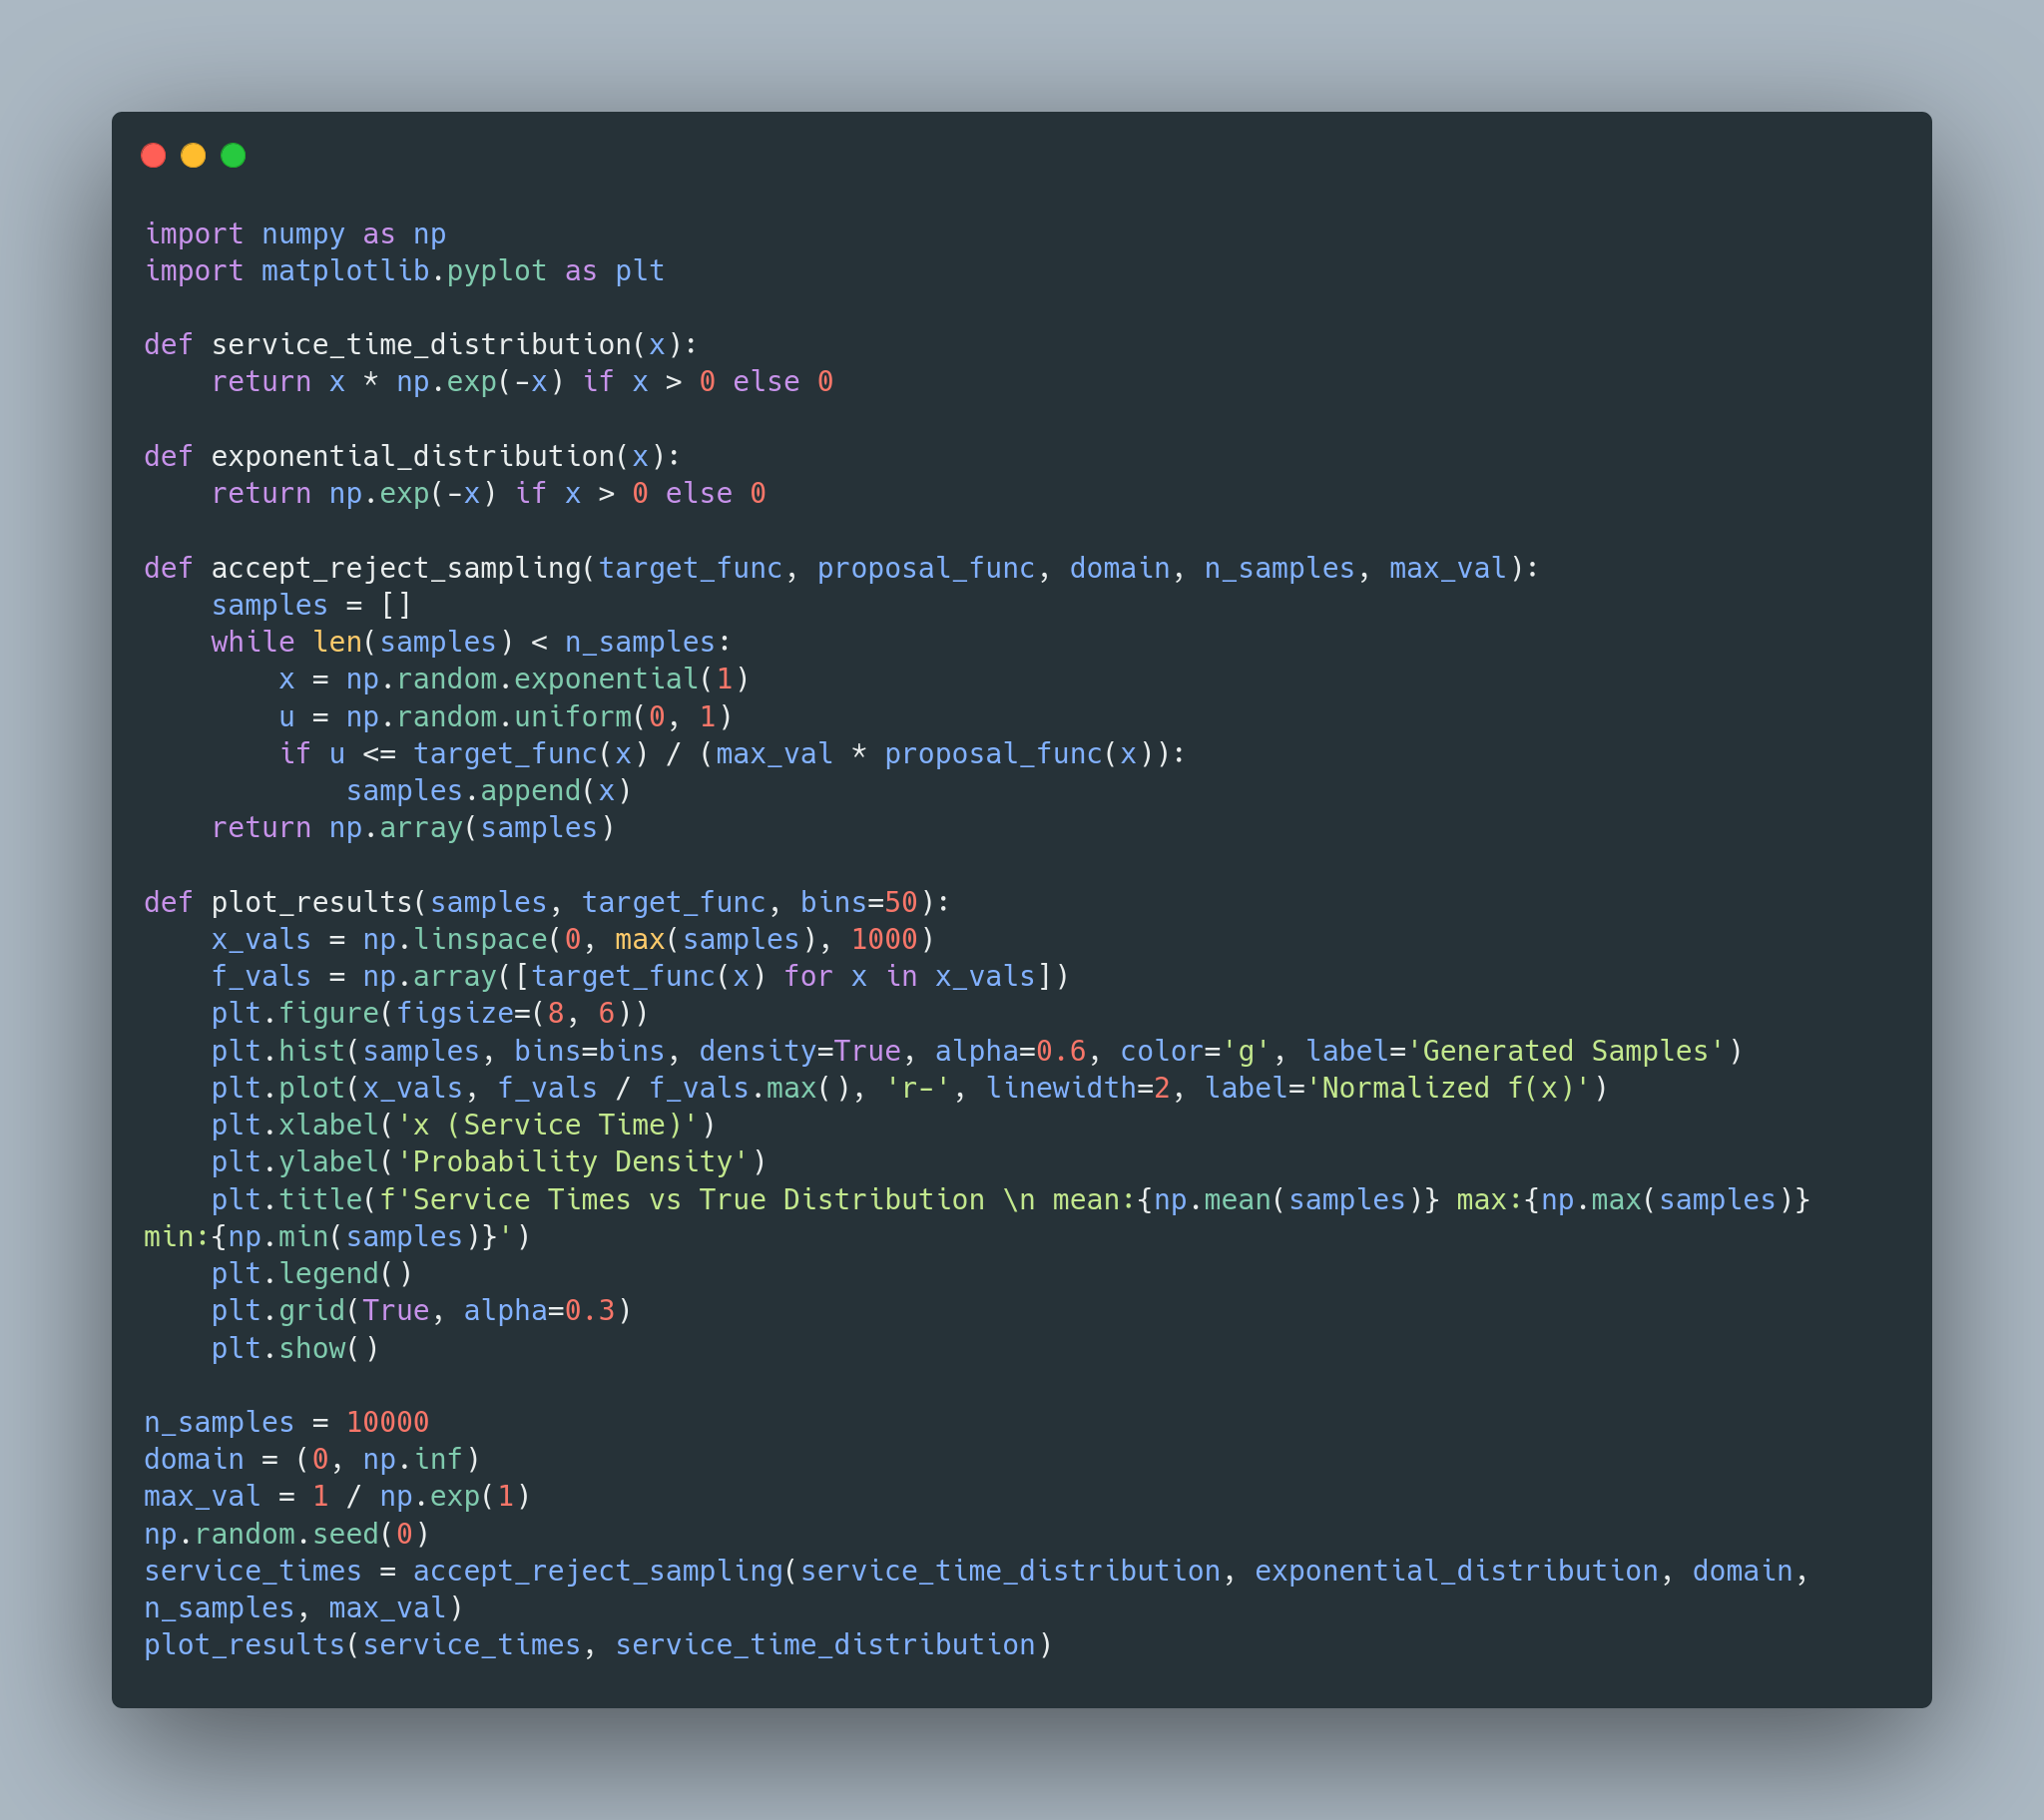
\includegraphics[width=0.6\textwidth]{./Screenshots/3.py.png} 
\end{figure} \\
\begin{figure}[h!]
    \centering
    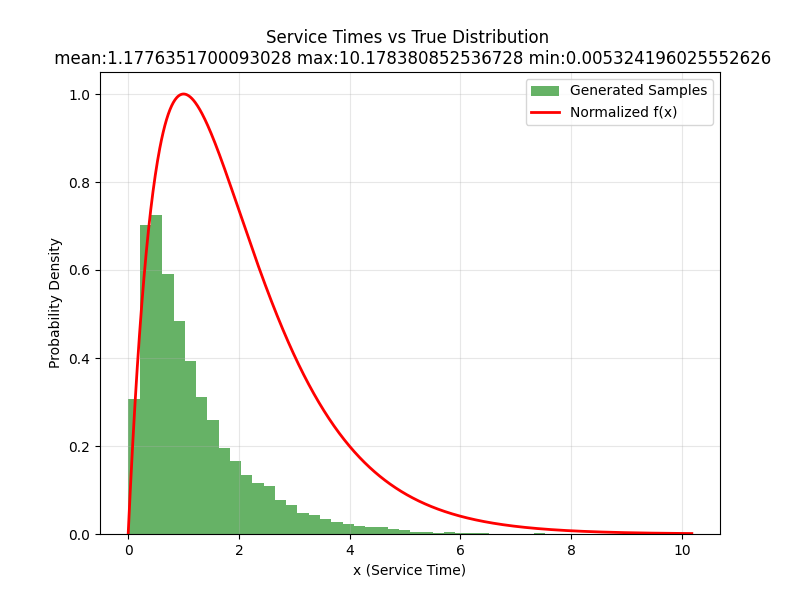
\includegraphics[width=0.6\textwidth]{./Screenshots/3.png} 
\end{figure} 
\newpage

\section{Exercise 4}
Generate random numbers for a triangular distribution defined on $[a, b]$ with mode $c$.
\begin{figure}[h!]
    \centering
    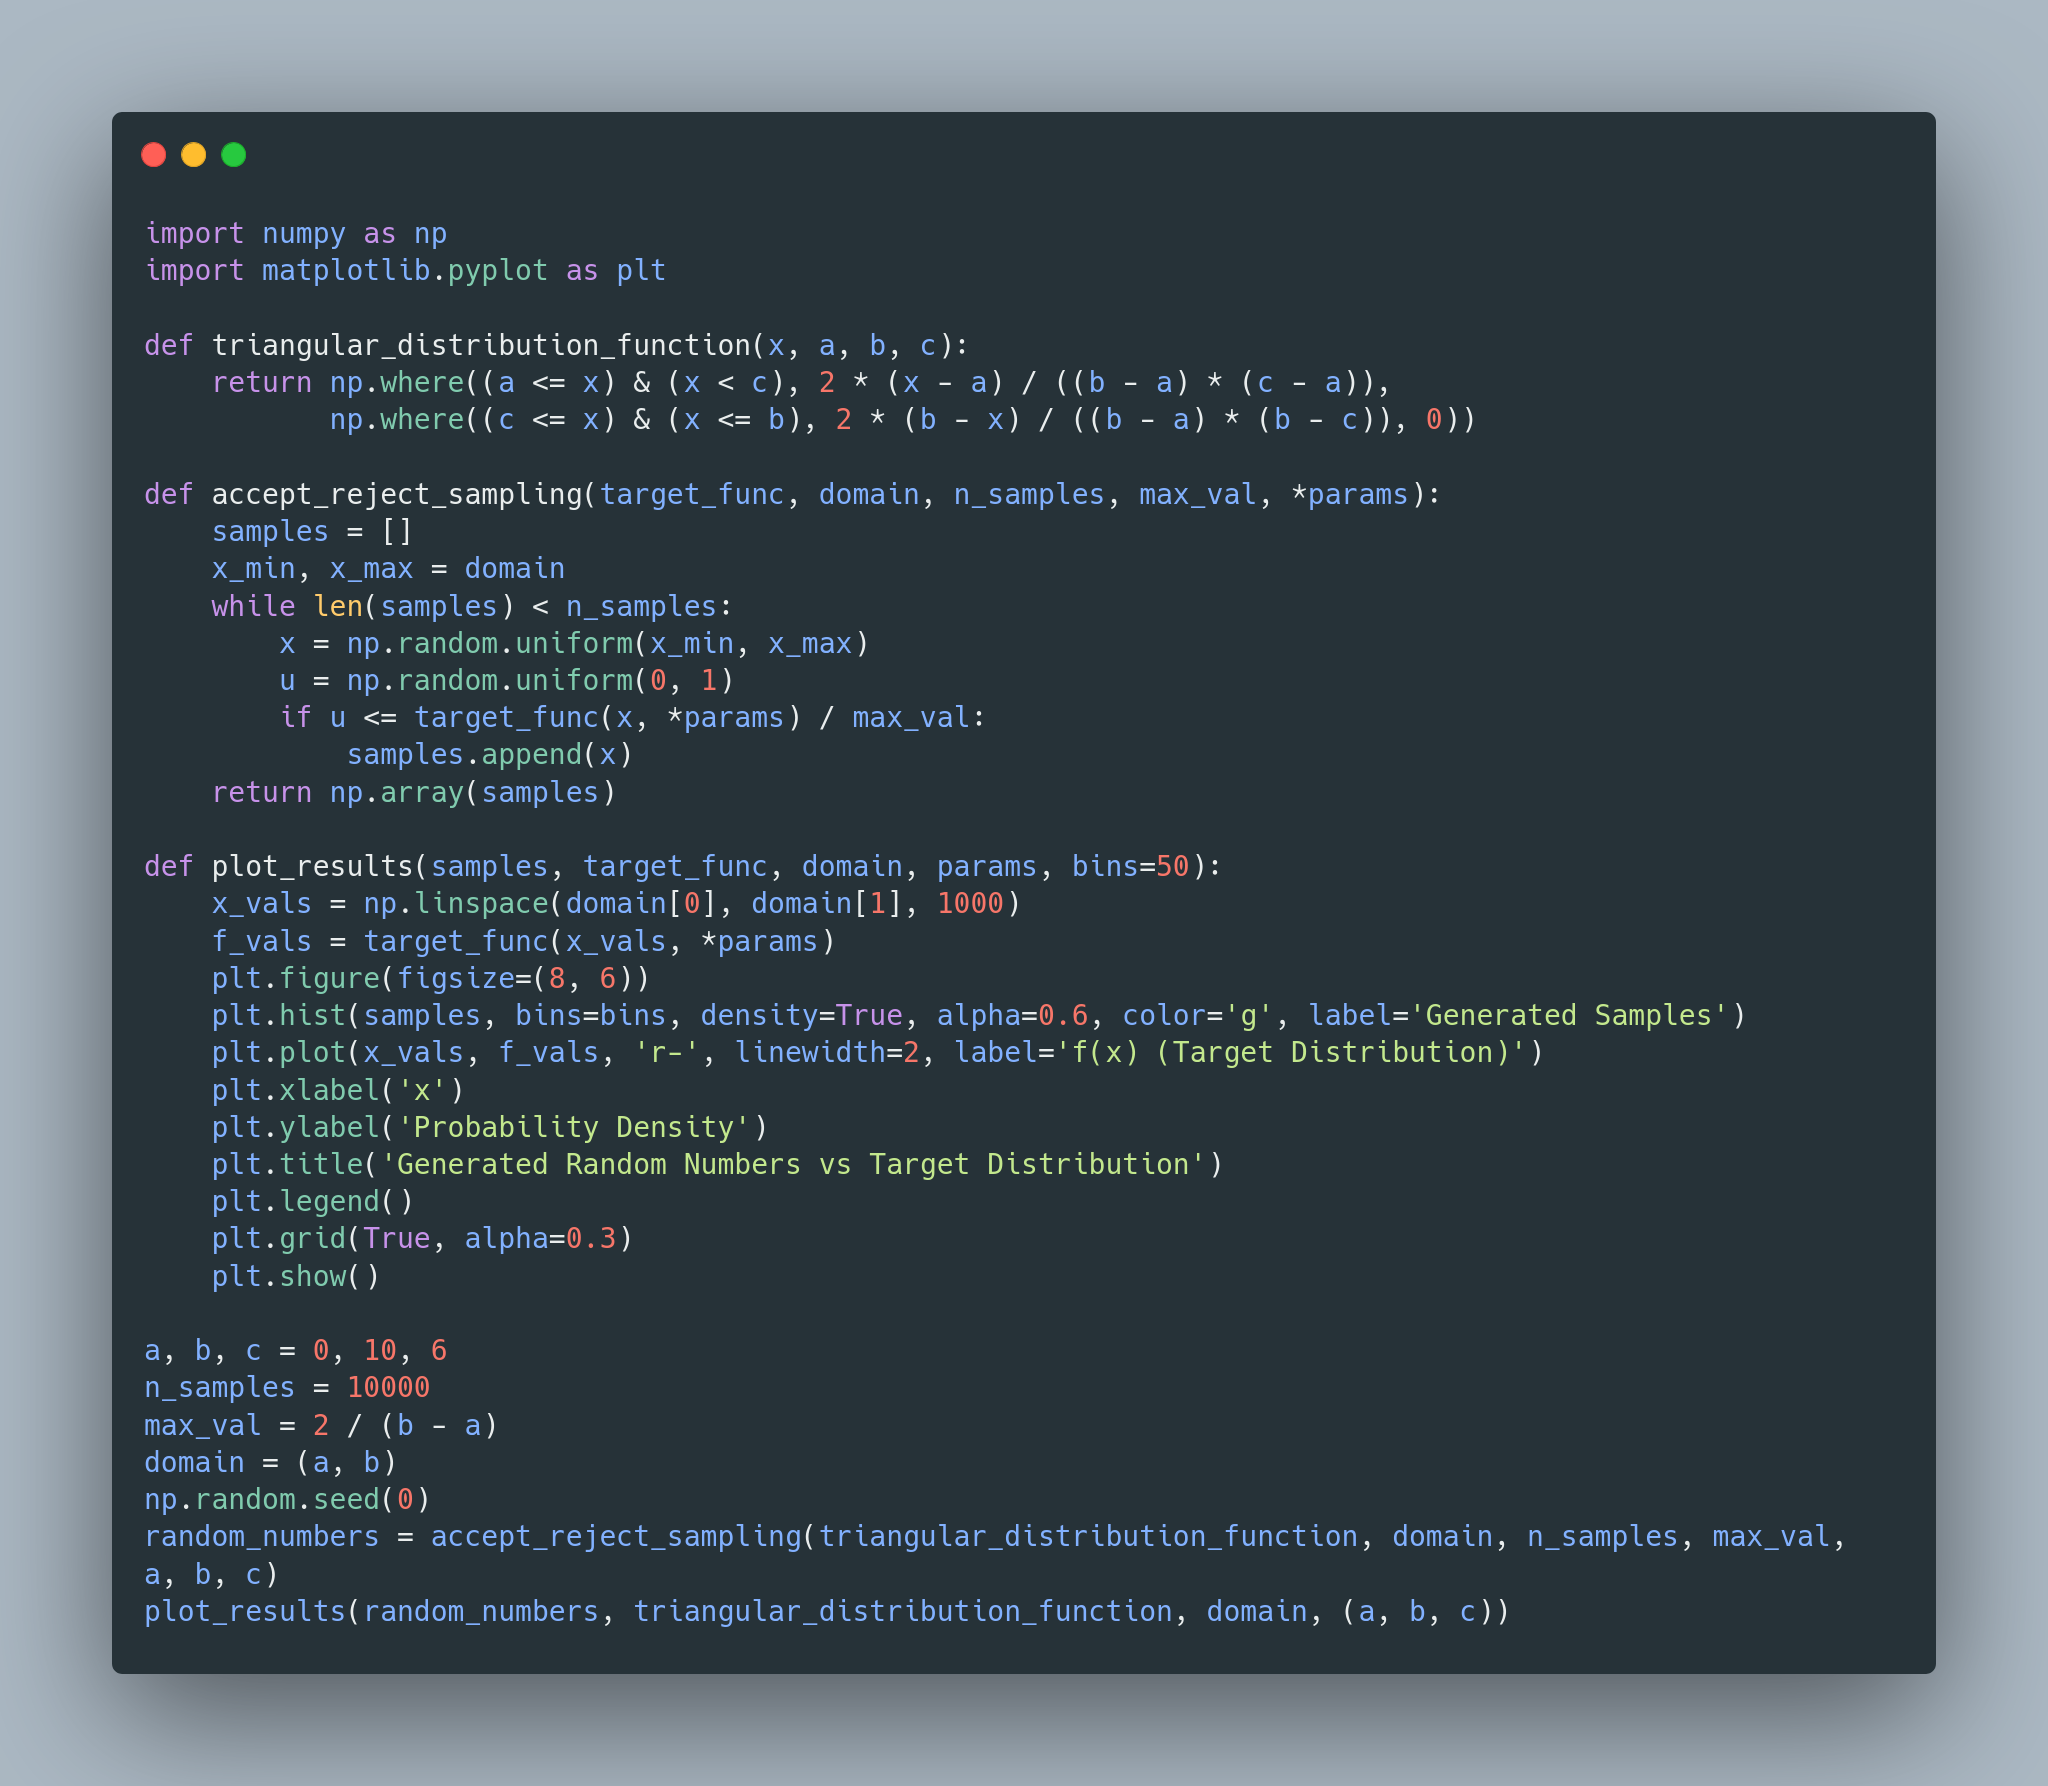
\includegraphics[width=0.6\textwidth]{./Screenshots/4.py.png} 
\end{figure} \\
\begin{figure}[h!]
    \centering
    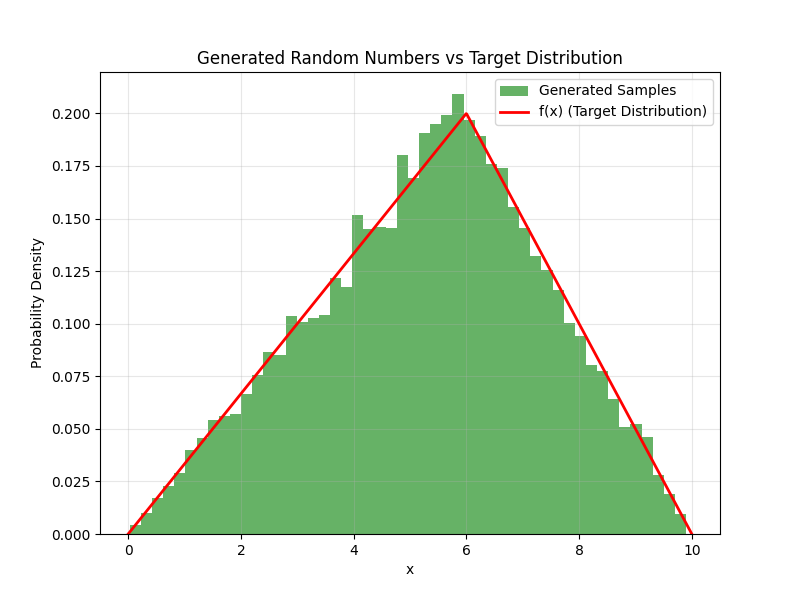
\includegraphics[width=0.6\textwidth]{./Screenshots/4.png} 
\end{figure} 
\newpage

\section{Exercise 5}
Implement a random number generator for the Rayleigh distribution with variance $\sigma^2$.

\\ The Rayleigh distribution is a continuous probability distribution commonly used in signal processing, radar systems, and various statistical applications.
\[
PDF: f(x; \sigma) = \frac{x}{\sigma^2} e^{-\frac{x^2}{2\sigma^2}}, \quad x \geq 0,
\]
\[
CDF: F(x; \sigma) = 1 - e^{-\frac{x^2}{2\sigma^2}}, \quad x \geq 0.
\]
\begin{figure}[h!]
    \centering
    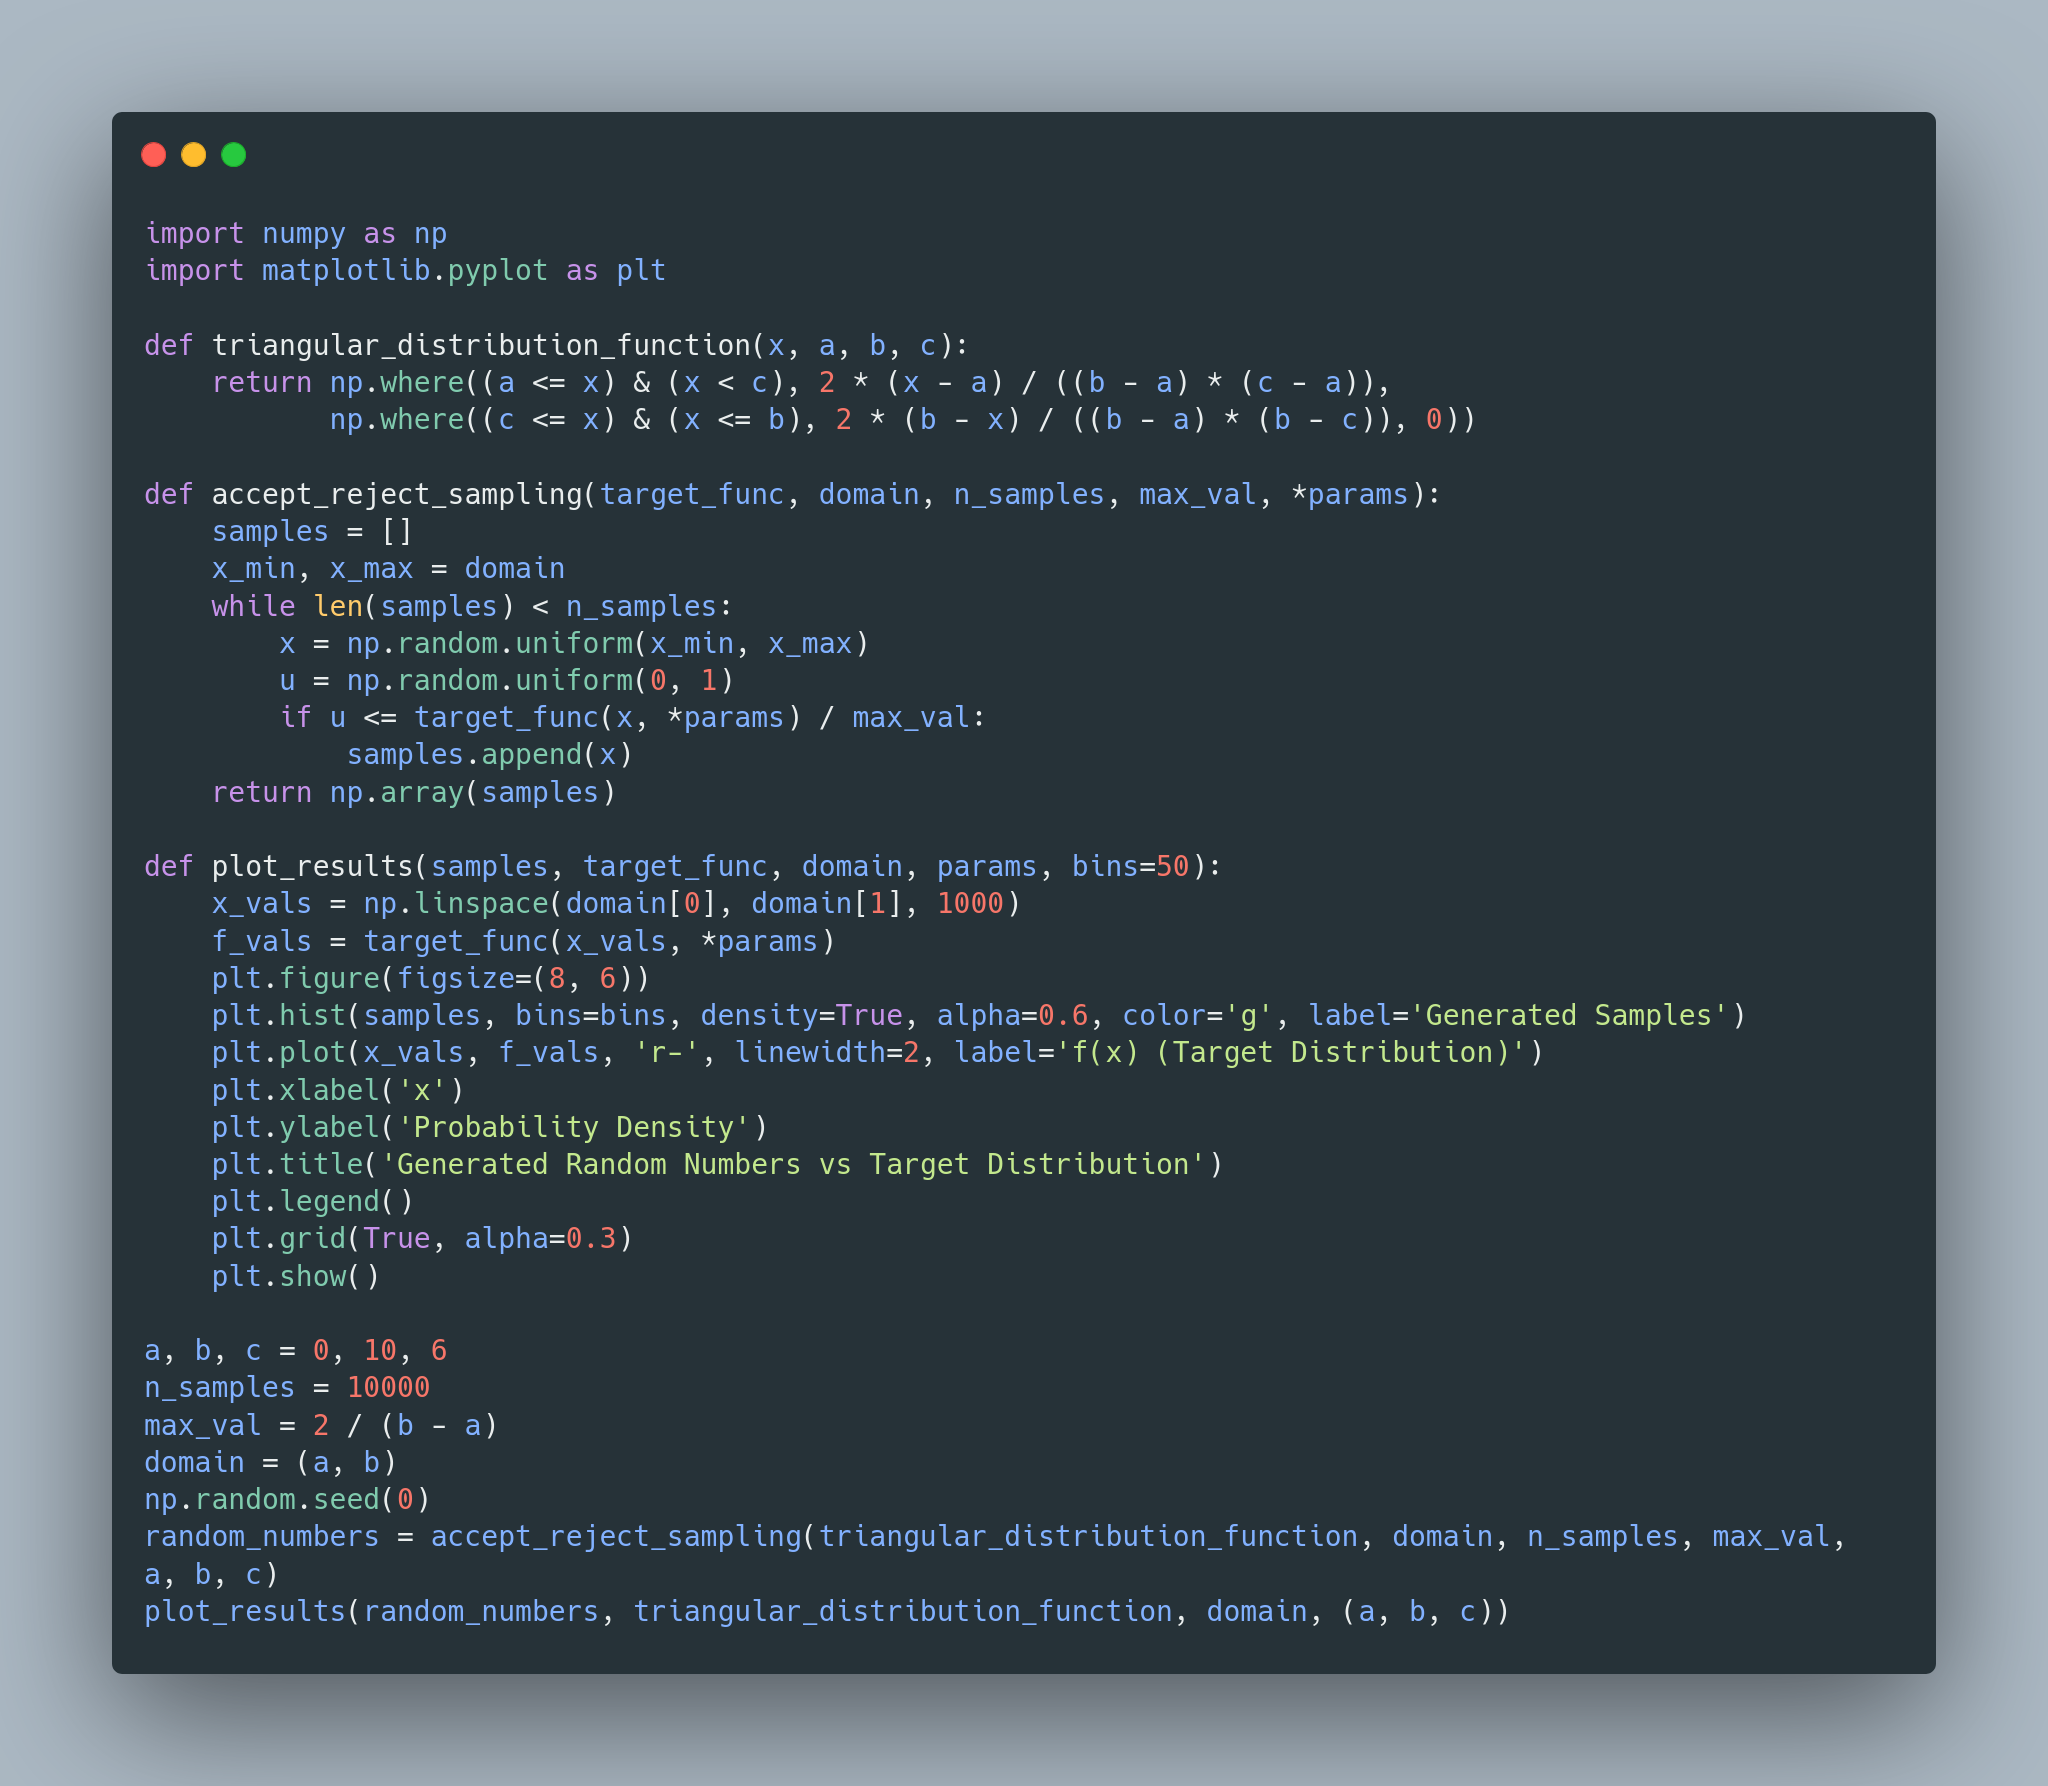
\includegraphics[width=0.6\textwidth]{./Screenshots/4.py.png} 
\end{figure} \\
\begin{figure}[h!]
    \centering
    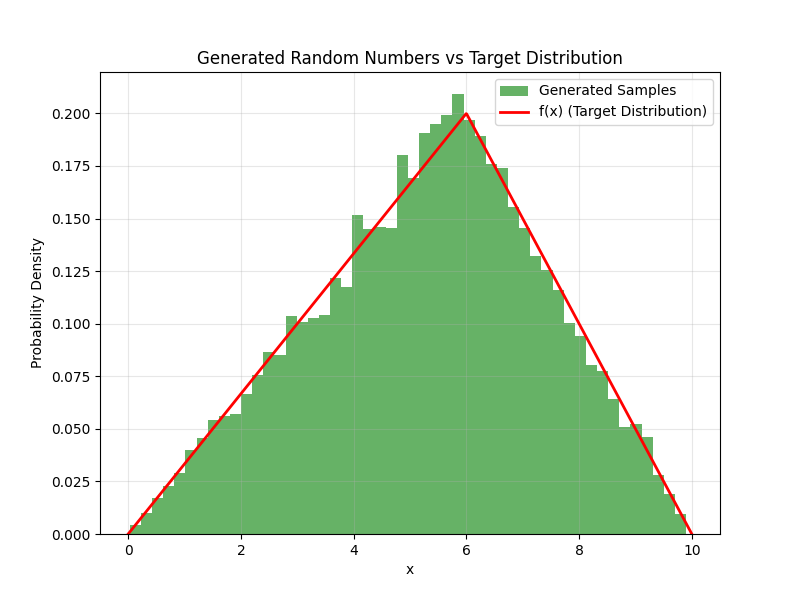
\includegraphics[width=0.5\textwidth]{./Screenshots/4.png} 
\end{figure} 
\newpage
\section{Exercise 6}
Simulate a bank with multiple counters where:
\begin{itemize}
    \item Customer arrival times follow an exponential distribution.
    \item Service times at counters also follow an exponential distribution.
\end{itemize}
\begin{figure}[h!]
    \centering
    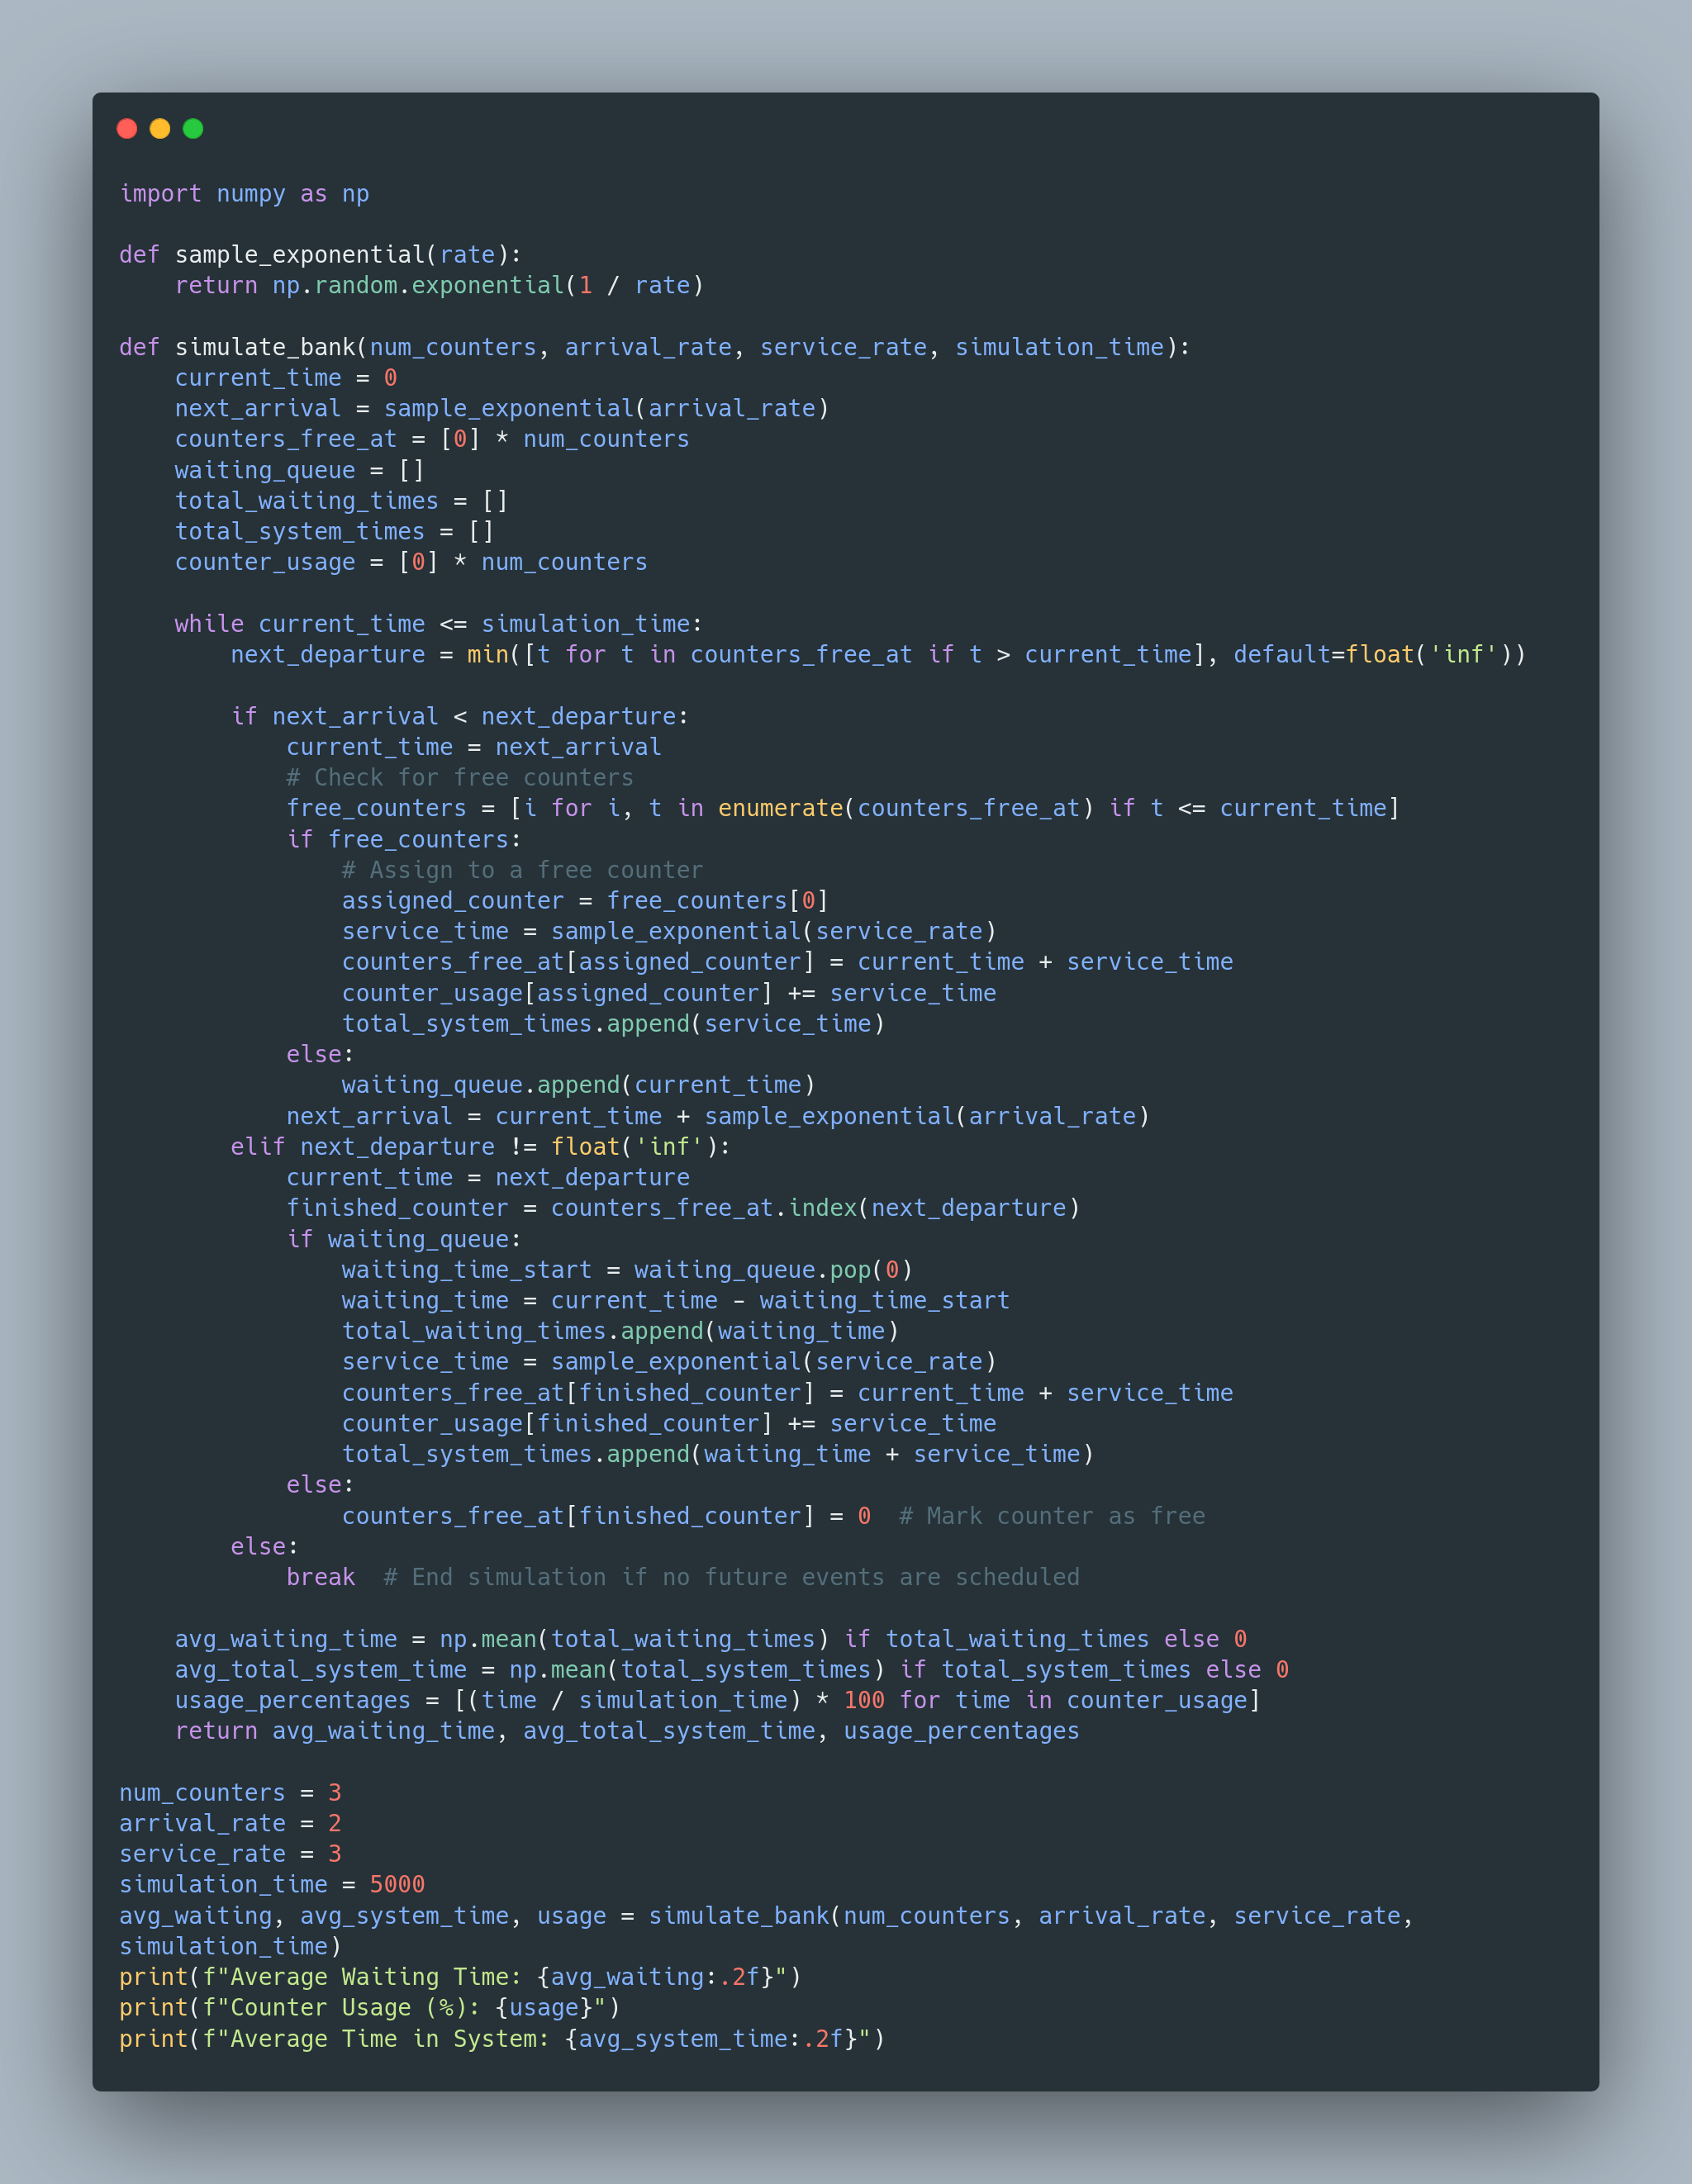
\includegraphics[width=0.5\textwidth]{./Screenshots/6.py.png}
\end{figure}
The simulation was conducted using the following input parameters:
\begin{itemize}
    \item Number of Counters: 3
    \item Arrival Rate (\(\lambda_a\)): 2 customers per unit time
    \item Service Rate (\(\lambda_s\)): 3 customers per unit time
    \item Simulation Time: 5000 time units
\end{itemize}
Based on the input parameters, the simulation produced the following results:
\begin{itemize}
    \item Average Waiting Time: 0.14 time units.
    \item Counter Usage: 40.03\% ,  19.41\% ,6.67\% 
    \item Average Time in System: 0.34 time units.
\end{itemize}
\newpage
\section{Exercise 7}

\begin{figure}[h!]
    \centering
    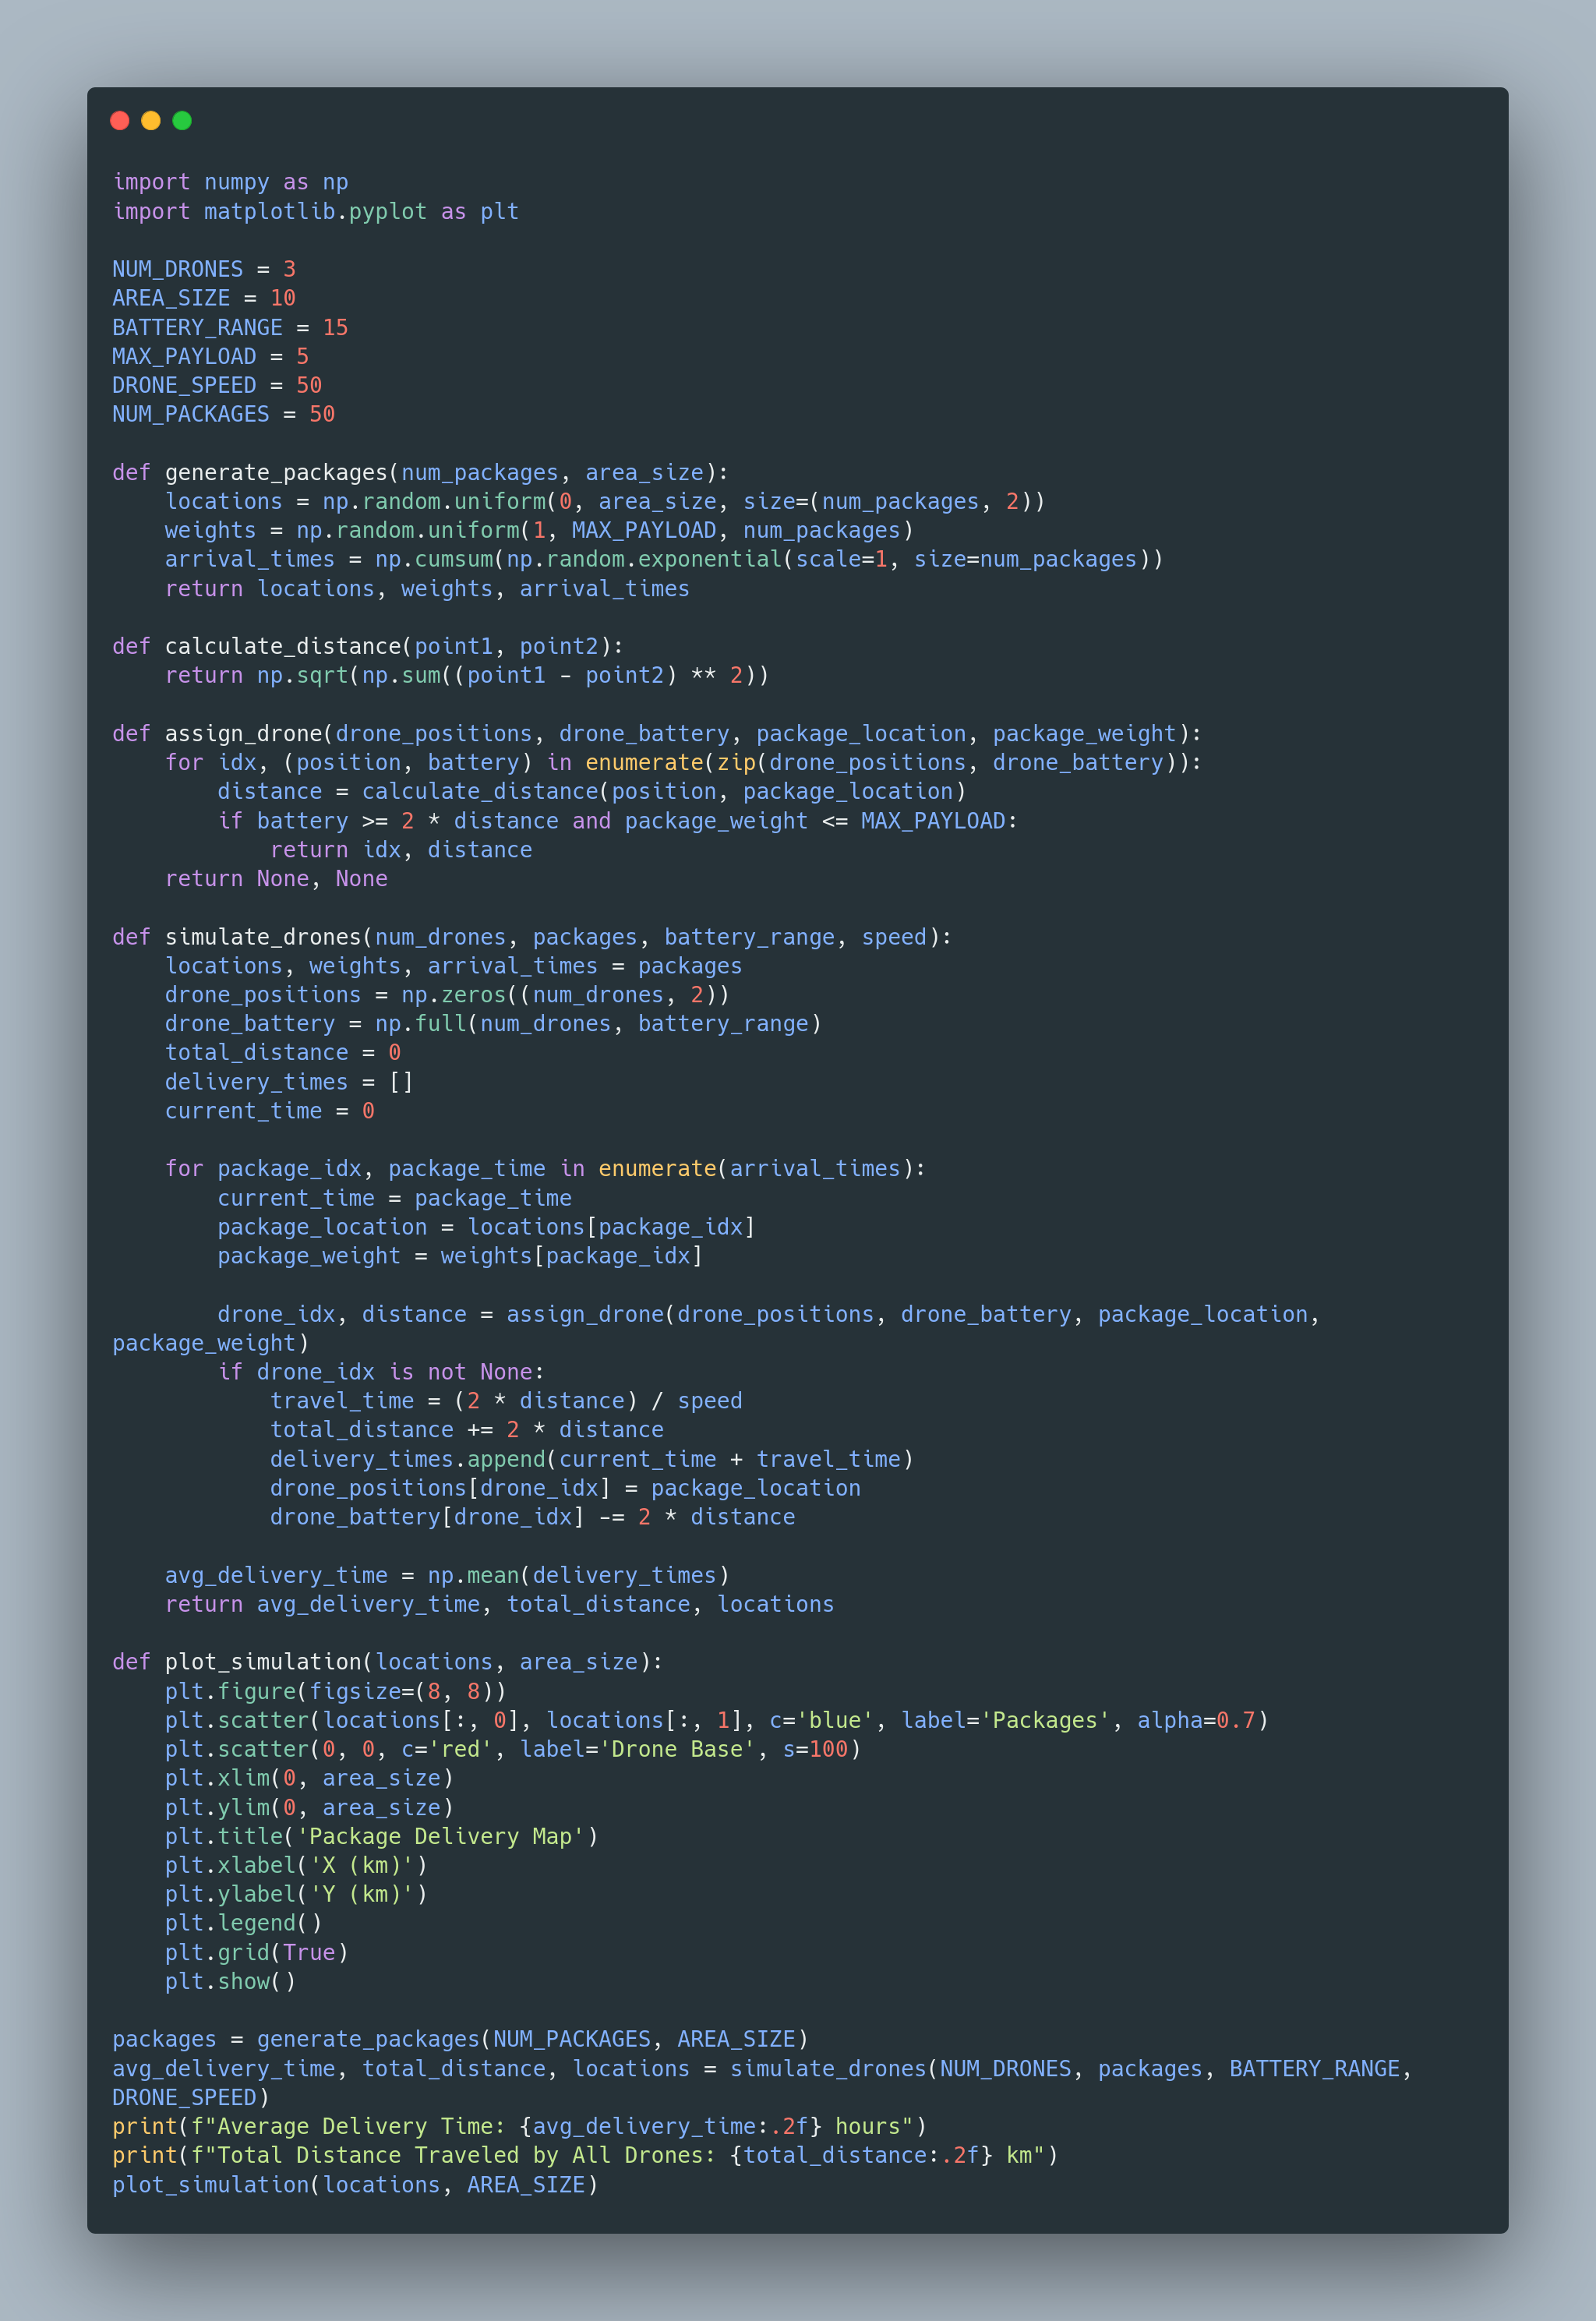
\includegraphics[width=0.5\textwidth]{./Screenshots/7.py.png} 
\end{figure} \\
\begin{figure}[h!]
    \centering
    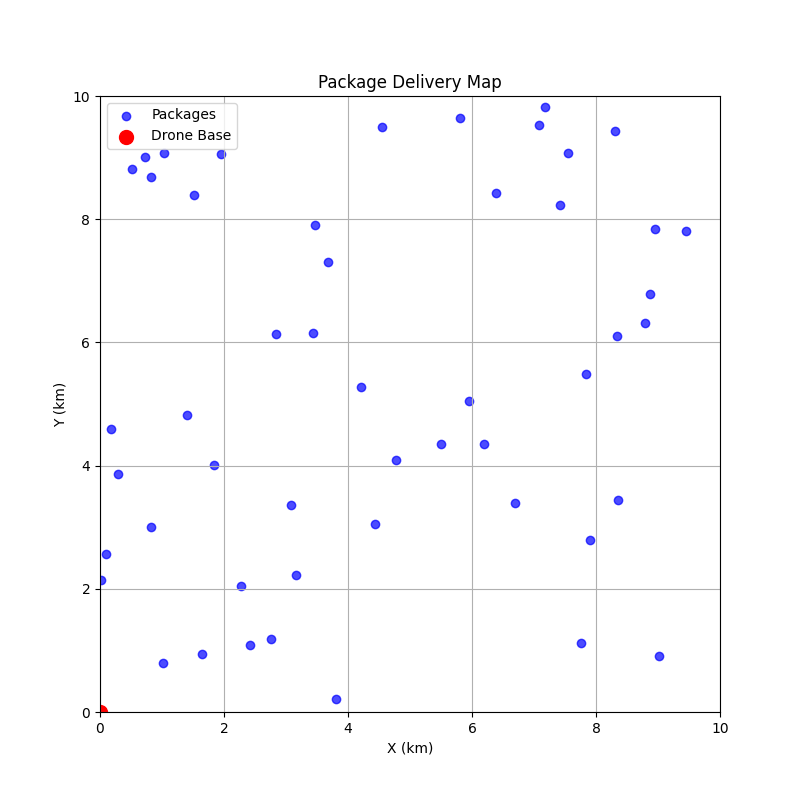
\includegraphics[width=0.5\textwidth]{./Screenshots/7.png} 
\end{figure} 
\begin{itemize}
    \item Average Delivery Time: 11.06 hours
    \item Total Distance Traveled by All Drones: 41.04 km 
\end{itemize}
\end{enumerate}
\end{document}
